%%%%%%%%%%%%%%%%%%%%%%%%%%%%%%%%%%%%%%%%%
% fphw Assignment
% LaTeX Template
% Version 1.0 (27/04/2019)
%
% This template originates from:
% https://www.LaTeXTemplates.com
%
% Authors:
% Class by Felipe Portales-Oliva (f.portales.oliva@gmail.com) with template 
% content and modifications by Vel (vel@LaTeXTemplates.com)
%
% Template (this file) License:
% CC BY-NC-SA 3.0 (http://creativecommons.org/licenses/by-nc-sa/3.0/)
%
%%%%%%%%%%%%%%%%%%%%%%%%%%%%%%%%%%%%%%%%%

%----------------------------------------------------------------------------------------
%	PACKAGES AND OTHER DOCUMENT CONFIGURATIONS
%----------------------------------------------------------------------------------------

\documentclass[
	french,
	11pt, % Default font size, values between 10pt-12pt are allowed
	%letterpaper, % Uncomment for US letter paper size
	%spanish, % Uncomment for Spanish
]{fphw}

% Template-specific packages
\usepackage{babel}
\usepackage[utf8]{inputenc} % Required for inputting international characters
\usepackage[T1]{fontenc} % Output font encoding for international characters
\usepackage{mathpazo} % Use the Palatino font
% \usepackage{iwona} % Use the Iwona font

\usepackage{amsmath}
\usepackage{mathtools}
\usepackage{xfrac} 

\usepackage{graphicx} % Required for including images
\usepackage[textfont=it]{caption}  %% To manage long captions in images
\usepackage{subcaption}
\captionsetup{justification=centering}
\captionsetup[table]{position=bottom}
\newcommand{\tabhead}[1]{{\bfseries#1}}

\usepackage{subcaption}
\usepackage{float}
\graphicspath{ {./img/} }

\usepackage{booktabs} % Required for better horizontal rules in tables

\usepackage{xcolor}
\usepackage{listings}
\colorlet{mygray}{black!30}
\colorlet{mygreen}{green!60!blue}
\colorlet{mymauve}{red!60!blue}
\lstset{
  backgroundcolor=\color{gray!10},  
  basicstyle=\scriptsize\ttfamily,
  columns=fullflexible,
  breakatwhitespace=false,      
  breaklines=true,                
  captionpos=b,                    
  commentstyle=\color{mygreen}, 
  extendedchars=true,              
  frame=single,                   
  keepspaces=true,             
  keywordstyle=\color{blue},      
  language=c++,                 
  numbers=none,                
  numbersep=5pt,                   
  numberstyle=\tiny\color{blue}, 
  rulecolor=\color{mygray},        
  showspaces=false,               
  showtabs=false,                 
  stepnumber=5,                  
  stringstyle=\color{mymauve},    
  tabsize=3,                      
  title=\lstname                
}

\usepackage[linkcolor=blue,colorlinks=true]{hyperref}
\usepackage{cleveref}

\usepackage{array} % Required for spacing in tabular environment

\usepackage{enumerate} % To modify the enumerate environment

\usepackage{amssymb}
\usepackage{enumitem}	%% % To modify the itemize bullet character

\newcommand{\hquad}{\hspace{0.5em}} %% Bew command for half quad
% \setlength\parindent{0pt}	%% To remove all indentations

\setlength\parindent{0pt}

%----------------------------------------------------------------------------------------
%	ASSIGNMENT INFORMATION
%----------------------------------------------------------------------------------------

\title{TP \#1} % Assignment title

\author{Roussel Desmond Nzoyem} % Student name

\date{\today} % Due date

\institute{Université de Strasbourg \\ UFR de Mathématiques et Informatique} % Institute or school name

\class{EDP 2} % Course or class name

\professor{Pr. Philippe Helluy} % Professor or teacher in charge of the assignment

%----------------------------------------------------------------------------------------

\begin{document}

\maketitle % Output the assignment title, created automatically using the information in the custom commands above

%----------------------------------------------------------------------------------------
%	ASSIGNMENT CONTENT - SECTION 1
%----------------------------------------------------------------------------------------


\section{Résolution numérique de l'équation de transport}

\subsection*{Question 1.}
\begin{problem}
	Calculer la solution du problème suivant ($c$ est une constante $> 0$).
	\begin{align*}
		\begin{dcases}
			\partial_t u + c \partial_x u = 0, \quad x \in ]0, L[, \quad t \in ]0,T[ \\
			u(0, t) = e^{-t}, \quad t \in ]0,T[ \\
			u(x, 0) = 0, \quad x \in ]0,L[
		\end{dcases}
	\end{align*}
\end{problem}


\subsection*{Réponse} 

Nous procéderons par la méthode des courbes caractéristiques. Une courbe caractéristique est une courbe $t \mapsto {x(t) \choose t}$ telle que la solution $u(x(t),t)$ y soit constante. Pour l'équation de transport à résoudre, les courbes caractéristiques sont des droites du plan de coefficient directeur $c > 0$. 
Calculons la solution du problème.

\begin{itemize}[label=$\blacksquare$]
	\item Dans un premier temps, pour tout $y \in \mathbb{R}$, on a:
$$
\frac{d}{dt} u(y+ct, t) = \left( \frac{\partial u}{\partial t} + c \frac{\partial u}{\partial x}\right)(y+ct,t)=0, \qquad 0 < y+ct < L, \quad 0 < t < T 
$$
C'est à dire 
$$u(y+ct, t) = \text{Cste}, \qquad 0 < y+ct < L, \quad 0 < t < T$$
On choisi la constante correspondant au cas limite $t=0$
$$
u(y+ct, t) = u(y,0) \quad $$
sous les conditions suivantes
\begin{itemize}
	\item 
	$
	\begin{dcases}
		0 < y+ct < L \\
		0 < y < L
	\end{dcases}
	$ $ \Longrightarrow ct < y+ct < L $
	\item $0 < t < T$
\end{itemize}  
On effectue le changement de variable $y+ct = x$ pour obtenir la solution 
$$u(x, t) = 0$$ 
définie sur l'ensemble:
$$
\left\{ (x,t) \in ]0, L[ \times ]0, T[ \quad \text{tel que} \quad ct < x \right\}
$$

\item 

D'autre part, pour tout $t^\prime > 0$, on a:
$$
\frac{d}{ds} u(cs, t^\prime + s) = \left( \frac{\partial u}{\partial t} + c \frac{\partial u}{\partial x}\right)(cs, t^\prime + s)=0, \quad 0 < cs < L, \quad 0 < t^\prime + s < T 
$$
C'est à dire
$$u(cs, t^\prime + s) = \text{Cste}, \quad 0 < cs < L, \quad 0 < t^\prime + s < T $$
On choisi la constante correspondant à $s=0$: 
$$u(cs, t^\prime + s) = u(0, t^\prime), \quad 0 < cs < L, \quad s < t^\prime + s < T $$
On effectue le changement de variable $$
	\begin{dcases}
		x = cs \\
		t = t^\prime + s
	\end{dcases} 
	\Longrightarrow t^\prime = t - \frac{x}{c} $$   
Ceci permet d'écrire
$$ u(x,t) = u(0, t - \frac{x}{c}) = e^{-t + \frac{x}{c}}$$ 
Sachant que $t^\prime > 0$ (car $t^\prime +s > s$), la solution donnée est définie sur:
$$\left\{ (x,t) \in ]0, L[ \times ]0, T[ \quad \text{tel que} \quad \frac{x}{c} < t \right\}$$

\end{itemize}

On récapitule en écrivant la solution de l'équation de transport

$$
\text{Pour} \, x \in ]0, L[ \text{  et  } t \in ]0, T[, \hquad u(x,t) = 
\begin{dcases}
	0 & \quad \text{si} \quad  ct < x\\
	e^{-t + \frac{x}{c}} & \quad \text{si} \quad ct > x
\end{dcases} 
$$

\begin{figure}[h]
	\centering
	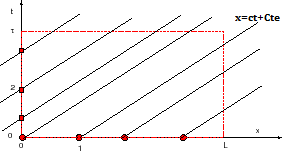
\includegraphics[width=0.5\textwidth]{Transport1}
	\captionsetup{justification=centering}
	\caption{Illustration de la solution de l'équation de Transport dans l'espace-temps à l'aide des courbes caractéristiques.}
\end{figure}

%--------------------------------------------------------------------------------------

\subsection*{Question 2.}
\begin{problem}
	Montrer que le problème n'admet pas de solution lorsque $c < 0$.
\end{problem}

\subsection*{Réponse} 

Procédons par l'absurde et supposons que le problème admette une solution $u(\cdot,\cdot)$.

\noindent Soit $x \in ]0, L[\, \text{et} \, t \in ]0, T[$. Pour tout $s \in \mathbb{R}$, on a: 
$$
\frac{d}{ds} u(x+cs, t+s) = \left( \frac{\partial u}{\partial t} + c \frac{\partial u}{\partial x}\right)(x+cs, t+s)=0 
$$
Avec $s$ t.q.
$
\begin{dcases}
	0 < x+cs < L \\
	0 < t+s < T
\end{dcases}  
\Rightarrow 
\begin{dcases}
	-L < cs < L \\
	-T < s < T
\end{dcases}  
\Rightarrow 
s \in K = ]-\min(T, -\frac{L}{c}), \min(T, -\frac{L}{c})[
$

\noindent On obtient donc: 
\begin{equation}
	\forall \, s \in K \quad u(x+cs, t+s) = \text{Cste} 
	\label{uCste}
\end{equation}
En particulier, pour $s=0 \in K$, on a $u(x+cs, t+s) = u(x, t)$ 

\begin{itemize}[label=$\blacksquare$]
	\item  Supposons $-\frac{L}{c} < T \,\, \text{i.e.} \,\, K = ]\frac{L}{c}, -\frac{L}{c}[$; alors en prenant $s=-\frac{x}{c} \in K$, on a d'après (\refeq{uCste}):
	$$u(x+cs, t+s) = u(x, t) = u(0, t-\frac{x}{c})$$ 
	On constate déjà que la condition sur la borne gauche du domaine permet de définir entièrement l'évolution de $u$ (sans tenir compte de la condition initiale). 
	On peut relier les deux conditions aux limites en posant $x=-ct^\prime \hquad \text{et} \hquad t=0 $:
	\begin{itemize}
		\item D'une part $\quad u(x,t) = u(0, t-\frac{x}{c}) = u(0, t^\prime) = e^{-t^\prime}$
		\item D'autre part $\quad u(x,t) = u(-ct', 0) = 0$
	\end{itemize}
	Ceci pour tout $t^\prime \in ]0,-\frac{L}{c}[ $. Ce qui est absurde car $\hquad e^{-t^\prime} \neq 0 \quad \text{pour tout} \quad t^\prime \in \mathbb{R}$.

	\item Supposons au contraire $-\frac{L}{c} \geq T \,\, \text{i.e.} \,\, K = ]-T, T[$; on prends alors $s=-t \in K$, ce qui donne (d'après l'équation (\refeq{uCste})): 
	$$u(x+cs, t+s) = u(x, t) = u(x-ct, 0)$$
	Posons $x=0 \hquad \text{et} \hquad t=-\frac{x^\prime}{c} $:
	\begin{itemize}
		\item D'une part $\quad u(x, t) = u(x-ct, 0) = u(x^\prime, 0) = 0$
		\item D'autre part $\quad u(x,t) = u(0, -\frac{x^\prime}{c}) = e^{\frac{x^\prime}{c}}$
	\end{itemize}
	Ceci pour tout $x^\prime \in ]0,-cT[$. Ce qui est absurde!
\end{itemize}
Dans les deux cas, on constate que le problème n'admet pas de solution. D'un point de vue physique, ce résultat était attendu. Ceci car pour $c<0$, le transport de la quantité $u$ se fait de la droite vers la gauche. Au lieu d'imposer la condition sur le bord gauche ($x=0$), il aurait donc fallu fournir une condition sur le bord droit du domaine ($x=L$) pour que l'équation de transport admette une solution.


%-------------------------------------------------------------------------------

\subsection*{Question 3.}
\begin{problem}
	Écrire un programme qui résout l'équation de transport par la méthode de Godunov.
\end{problem}

\subsection*{Réponse}
Pour programmer la méthode de Godunov, il nous faut introduire certaines fonctions. Pour l'équation de transport, on les définit de la manière suivante:
\begin{itemize}
	\item Le flux physique: 
	% \begin{verbatim}
	\footnotesize
	\begin{lstlisting}[language=C]
	void fluxphy(double* w, double* flux) { flux[0] = _C * w[0]; }
	\end{lstlisting}
	\normalsize
	\item La vitesse maximale sur chaque cellule: 
	\footnotesize
	\begin{lstlisting}[language=C]
	double lambda_max(double* u) { return _C; }
	\end{lstlisting}
	\normalsize
	\item La solution du problème de Riemann associé: 
	\footnotesize
	\begin{lstlisting}[language=C]
	void riemann(double* a, double* b, double z, double* w) {
		if (z < _C) {       	// z = x/t
			w[0] = a[0];
		} else {
			w[0] = b[0];
		}
	}
	\end{lstlisting}
	\normalsize
	\item Une solution exacte du problème: utilisé comme condition initiale ($t=0$), et comme condition aux bords ($x=0$ et $x=L$): 
	\footnotesize
	\begin{lstlisting}[language=C]
	void solexacte(double x, double t, double* w) {
		double uR = 0;
		double uL = exp(-(t - x / _C));

		if (x < _C * t) {
			w[0] = uL;
		} else {
			w[0] = uR;
	}
	\end{lstlisting}
	\normalsize
	\item La fonction de résolution du problème, utilisable tel quel pour d'autres problèmes

	\begin{lstlisting}[language=C,breaklines]
	void godunov_solve(godunov* gd, double tmax) {
		double tnow = 0;
		int m = gd->m;
		while (tnow < tmax) {
			double vmax = 0;
			// Calcul de la vitesse max
			for (int i = 0; i < gd->N + 2; i++) {
				double vloc = lambda_max(gd->un + m * i);
				vmax = vmax > vloc ? vmax : vloc;
			}
			// Calcul du pas de temps
			gd->dt = gd->cfl * gd->dx / vmax;
			// Application du flux
			for (int i = 1; i < gd->N + 1; i++) {
				double flux[m];
				fluxnum(gd->un + i * m, gd->un + (i + 1) * m, flux);
				for (int iv = 0; iv < m; iv++) {
					gd->unp1[i * m + iv] =
						gd->un[i * m + iv] - gd->dt / gd->dx * flux[iv];
				} 
				fluxnum(gd->un + (i - 1) * m, gd->un + i * m, flux);
				for (int iv = 0; iv < m; iv++) {
					gd->unp1[i * m + iv] += gd->dt / gd->dx * flux[iv];
				}
			}
			// Mise à jour
			tnow += gd->dt;
			// Conditions aux limites
			int i = 0;
			solexacte(gd->xi[i], tnow, gd->unp1 + i * m);
			i = gd->N + 1;
			solexacte(gd->xi[i], tnow, gd->unp1 + i * m);
			// Preparation pour l'iteration suivante
			memcpy(gd->un, gd->unp1, (gd->N + 2) * m * sizeof(double));
		}
		gd->tfin = tnow;
	}		
	\end{lstlisting}	
\end{itemize}

On choisit de résoudre le problème avec $L = 2$, $T=0.7$, $c=1$ et $cfl$\footnote{Les détails sur le coefficient $cfl$ sont donnés à la question 5.}. Pour différents taille de maillage ($N=50, 1000, 50000$), on obtient les résultats suivants:

\begin{figure}[h]
	\centering
	\begin{subfigure}[b]{0.45\textwidth}
		\centering
		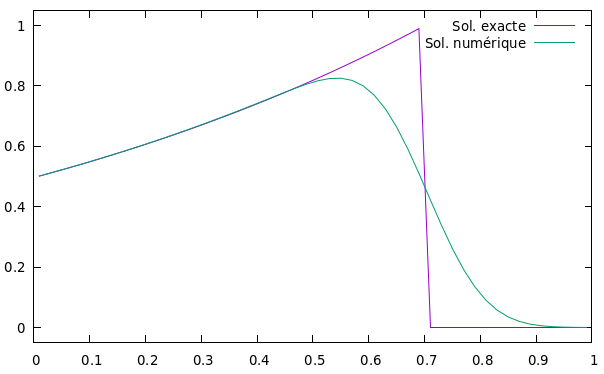
\includegraphics[width=\textwidth]{Transport50.png}
		\caption{$N=50$}
	\end{subfigure}
	% \hfill
	\begin{subfigure}[b]{0.45\textwidth}
		\centering
		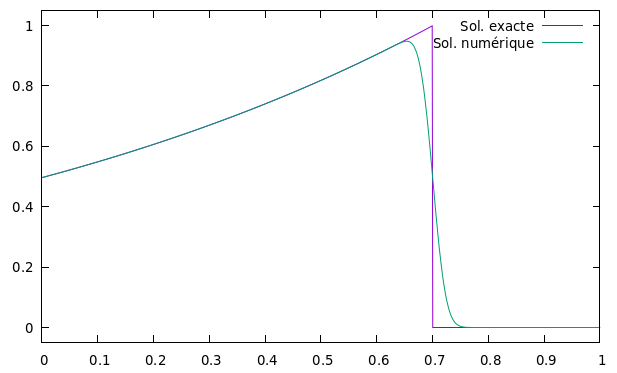
\includegraphics[width=\textwidth]{Transport1000.png}
		\caption{$N=1000$}
		\label{fig:Transportb}
	\end{subfigure}
	% \hfill
	\begin{subfigure}[b]{0.45\textwidth}
		\centering
		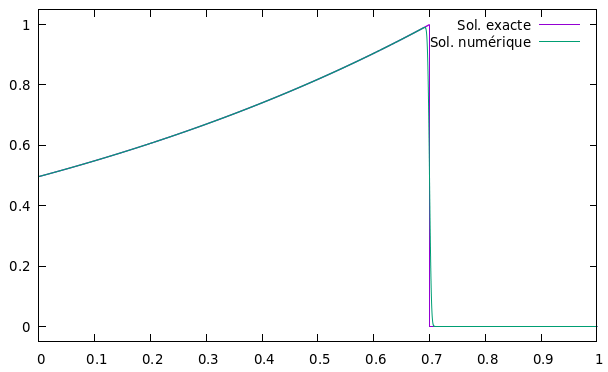
\includegraphics[width=\textwidth]{Transport50000.png}
		\caption{$N=50000$}
	\end{subfigure}
	% \hfill
	\captionsetup{justification=centering}
	\caption{Quelque résultats obtenus pour l'équation de transport au temps final $T=0.7$.}
\end{figure}


%-------------------------------------------------------------------------------

\subsection*{Question 4.}
\begin{problem}
	Étude du taux de convergence. Vérifions la validité de notre programme sur l'équation de transport en traçant le logarithme de l'erreur en norme $L^1$ entre la solution exacte à l'instant $T$ et la solution numérique en fonction de $\text{ln}(\Delta x)$ où $\Delta x$ est le pas de la subdivision.
\end{problem}

\subsection*{Réponse}
On obtient le tableau de convergence illustré ci-bas (\cref{table:Transport}); son illustration est donnée à la \cref{fig:TransportCvg}.

\begin{table}[h!]
	\centering
	\renewcommand{\arraystretch}{1.2}
	\begin{tabular}{| m{2cm} | m{2cm} | m{2cm} |} 
	\hline 
	\multicolumn{1}{|c|}{$N$} & \multicolumn{1}{|c|}{$\Delta x$} & \multicolumn{1}{|c|}{Erreur $L^1$} \\ [0.5ex] 
	\hline \hline
	% \toprule
	10 & 0.100000 & 0.140029 \\ [0.5ex]
	% \hline
	% \midrule
	40 & 0.025000 & 0.074383 \\ [0.5ex]
	% \hline
	160 & 0.006250 & 0.037323 \\ [0.5ex]
	% \hline
	640 & 0.001563 & 0.018697 \\ [0.5ex]
	% \hline
	2560 & 0.000391 & 0.009342 \\ [0.5ex] 
	% \hline
	10240 & 0.000098 & 0.004669 \\ [0.5ex] 
	\hline
	% \bottomrule
   \end{tabular}
	\caption{Étude de convergence pour l'équation de transport}
	\label{table:Transport}
\end{table}


\begin{figure}[H]
	\centering
	% \hspace*{0.9cm}
	\scalebox{.6}{% GNUPLOT: LaTeX picture with Postscript
\begingroup
  \makeatletter
  \providecommand\color[2][]{%
    \GenericError{(gnuplot) \space\space\space\@spaces}{%
      Package color not loaded in conjunction with
      terminal option `colourtext'%
    }{See the gnuplot documentation for explanation.%
    }{Either use 'blacktext' in gnuplot or load the package
      color.sty in LaTeX.}%
    \renewcommand\color[2][]{}%
  }%
  \providecommand\includegraphics[2][]{%
    \GenericError{(gnuplot) \space\space\space\@spaces}{%
      Package graphicx or graphics not loaded%
    }{See the gnuplot documentation for explanation.%
    }{The gnuplot epslatex terminal needs graphicx.sty or graphics.sty.}%
    \renewcommand\includegraphics[2][]{}%
  }%
  \providecommand\rotatebox[2]{#2}%
  \@ifundefined{ifGPcolor}{%
    \newif\ifGPcolor
    \GPcolortrue
  }{}%
  \@ifundefined{ifGPblacktext}{%
    \newif\ifGPblacktext
    \GPblacktexttrue
  }{}%
  % define a \g@addto@macro without @ in the name:
  \let\gplgaddtomacro\g@addto@macro
  % define empty templates for all commands taking text:
  \gdef\gplbacktext{}%
  \gdef\gplfronttext{}%
  \makeatother
  \ifGPblacktext
    % no textcolor at all
    \def\colorrgb#1{}%
    \def\colorgray#1{}%
  \else
    % gray or color?
    \ifGPcolor
      \def\colorrgb#1{\color[rgb]{#1}}%
      \def\colorgray#1{\color[gray]{#1}}%
      \expandafter\def\csname LTw\endcsname{\color{white}}%
      \expandafter\def\csname LTb\endcsname{\color{black}}%
      \expandafter\def\csname LTa\endcsname{\color{black}}%
      \expandafter\def\csname LT0\endcsname{\color[rgb]{1,0,0}}%
      \expandafter\def\csname LT1\endcsname{\color[rgb]{0,1,0}}%
      \expandafter\def\csname LT2\endcsname{\color[rgb]{0,0,1}}%
      \expandafter\def\csname LT3\endcsname{\color[rgb]{1,0,1}}%
      \expandafter\def\csname LT4\endcsname{\color[rgb]{0,1,1}}%
      \expandafter\def\csname LT5\endcsname{\color[rgb]{1,1,0}}%
      \expandafter\def\csname LT6\endcsname{\color[rgb]{0,0,0}}%
      \expandafter\def\csname LT7\endcsname{\color[rgb]{1,0.3,0}}%
      \expandafter\def\csname LT8\endcsname{\color[rgb]{0.5,0.5,0.5}}%
    \else
      % gray
      \def\colorrgb#1{\color{black}}%
      \def\colorgray#1{\color[gray]{#1}}%
      \expandafter\def\csname LTw\endcsname{\color{white}}%
      \expandafter\def\csname LTb\endcsname{\color{black}}%
      \expandafter\def\csname LTa\endcsname{\color{black}}%
      \expandafter\def\csname LT0\endcsname{\color{black}}%
      \expandafter\def\csname LT1\endcsname{\color{black}}%
      \expandafter\def\csname LT2\endcsname{\color{black}}%
      \expandafter\def\csname LT3\endcsname{\color{black}}%
      \expandafter\def\csname LT4\endcsname{\color{black}}%
      \expandafter\def\csname LT5\endcsname{\color{black}}%
      \expandafter\def\csname LT6\endcsname{\color{black}}%
      \expandafter\def\csname LT7\endcsname{\color{black}}%
      \expandafter\def\csname LT8\endcsname{\color{black}}%
    \fi
  \fi
    \setlength{\unitlength}{0.0500bp}%
    \ifx\gptboxheight\undefined%
      \newlength{\gptboxheight}%
      \newlength{\gptboxwidth}%
      \newsavebox{\gptboxtext}%
    \fi%
    \setlength{\fboxrule}{0.5pt}%
    \setlength{\fboxsep}{1pt}%
\begin{picture}(7200.00,5040.00)%
    \gplgaddtomacro\gplbacktext{%
      \csname LTb\endcsname%%
      \put(1078,704){\makebox(0,0)[r]{\strut{}$0.001$}}%
      \put(1078,2076){\makebox(0,0)[r]{\strut{}$0.01$}}%
      \put(1078,3447){\makebox(0,0)[r]{\strut{}$0.1$}}%
      \put(1078,4819){\makebox(0,0)[r]{\strut{}$1$}}%
      \put(1226,484){\makebox(0,0){\strut{}0.00010}}%
      \put(3085,484){\makebox(0,0){\strut{}0.00100}}%
      \put(4944,484){\makebox(0,0){\strut{}0.01000}}%
      \put(6803,484){\makebox(0,0){\strut{}0.10000}}%
    }%
    \gplgaddtomacro\gplfronttext{%
      \csname LTb\endcsname%%
      \put(209,2761){\rotatebox{90}{\makebox(0,0){\strut{}log(Erreur $L^1$)}}}%
      \put(4006,154){\makebox(0,0){\strut{}log($\Delta x$)}}%
      \csname LTb\endcsname%%
      \put(5816,4646){\makebox(0,0)[r]{\strut{}Pente = 0.48761}}%
    }%
    \gplbacktext
    \put(0,0){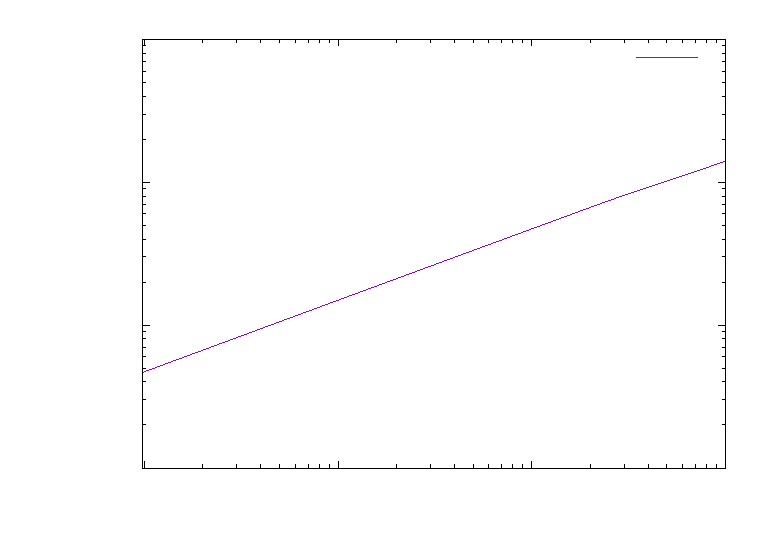
\includegraphics{TransportCvg}}%
    \gplfronttext
  \end{picture}%
\endgroup
}
	% \resizebox{.5\linewidth}{!}{% GNUPLOT: LaTeX picture with Postscript
\begingroup
  \makeatletter
  \providecommand\color[2][]{%
    \GenericError{(gnuplot) \space\space\space\@spaces}{%
      Package color not loaded in conjunction with
      terminal option `colourtext'%
    }{See the gnuplot documentation for explanation.%
    }{Either use 'blacktext' in gnuplot or load the package
      color.sty in LaTeX.}%
    \renewcommand\color[2][]{}%
  }%
  \providecommand\includegraphics[2][]{%
    \GenericError{(gnuplot) \space\space\space\@spaces}{%
      Package graphicx or graphics not loaded%
    }{See the gnuplot documentation for explanation.%
    }{The gnuplot epslatex terminal needs graphicx.sty or graphics.sty.}%
    \renewcommand\includegraphics[2][]{}%
  }%
  \providecommand\rotatebox[2]{#2}%
  \@ifundefined{ifGPcolor}{%
    \newif\ifGPcolor
    \GPcolortrue
  }{}%
  \@ifundefined{ifGPblacktext}{%
    \newif\ifGPblacktext
    \GPblacktexttrue
  }{}%
  % define a \g@addto@macro without @ in the name:
  \let\gplgaddtomacro\g@addto@macro
  % define empty templates for all commands taking text:
  \gdef\gplbacktext{}%
  \gdef\gplfronttext{}%
  \makeatother
  \ifGPblacktext
    % no textcolor at all
    \def\colorrgb#1{}%
    \def\colorgray#1{}%
  \else
    % gray or color?
    \ifGPcolor
      \def\colorrgb#1{\color[rgb]{#1}}%
      \def\colorgray#1{\color[gray]{#1}}%
      \expandafter\def\csname LTw\endcsname{\color{white}}%
      \expandafter\def\csname LTb\endcsname{\color{black}}%
      \expandafter\def\csname LTa\endcsname{\color{black}}%
      \expandafter\def\csname LT0\endcsname{\color[rgb]{1,0,0}}%
      \expandafter\def\csname LT1\endcsname{\color[rgb]{0,1,0}}%
      \expandafter\def\csname LT2\endcsname{\color[rgb]{0,0,1}}%
      \expandafter\def\csname LT3\endcsname{\color[rgb]{1,0,1}}%
      \expandafter\def\csname LT4\endcsname{\color[rgb]{0,1,1}}%
      \expandafter\def\csname LT5\endcsname{\color[rgb]{1,1,0}}%
      \expandafter\def\csname LT6\endcsname{\color[rgb]{0,0,0}}%
      \expandafter\def\csname LT7\endcsname{\color[rgb]{1,0.3,0}}%
      \expandafter\def\csname LT8\endcsname{\color[rgb]{0.5,0.5,0.5}}%
    \else
      % gray
      \def\colorrgb#1{\color{black}}%
      \def\colorgray#1{\color[gray]{#1}}%
      \expandafter\def\csname LTw\endcsname{\color{white}}%
      \expandafter\def\csname LTb\endcsname{\color{black}}%
      \expandafter\def\csname LTa\endcsname{\color{black}}%
      \expandafter\def\csname LT0\endcsname{\color{black}}%
      \expandafter\def\csname LT1\endcsname{\color{black}}%
      \expandafter\def\csname LT2\endcsname{\color{black}}%
      \expandafter\def\csname LT3\endcsname{\color{black}}%
      \expandafter\def\csname LT4\endcsname{\color{black}}%
      \expandafter\def\csname LT5\endcsname{\color{black}}%
      \expandafter\def\csname LT6\endcsname{\color{black}}%
      \expandafter\def\csname LT7\endcsname{\color{black}}%
      \expandafter\def\csname LT8\endcsname{\color{black}}%
    \fi
  \fi
    \setlength{\unitlength}{0.0500bp}%
    \ifx\gptboxheight\undefined%
      \newlength{\gptboxheight}%
      \newlength{\gptboxwidth}%
      \newsavebox{\gptboxtext}%
    \fi%
    \setlength{\fboxrule}{0.5pt}%
    \setlength{\fboxsep}{1pt}%
\begin{picture}(7200.00,5040.00)%
    \gplgaddtomacro\gplbacktext{%
      \csname LTb\endcsname%%
      \put(1078,704){\makebox(0,0)[r]{\strut{}$0.001$}}%
      \put(1078,2076){\makebox(0,0)[r]{\strut{}$0.01$}}%
      \put(1078,3447){\makebox(0,0)[r]{\strut{}$0.1$}}%
      \put(1078,4819){\makebox(0,0)[r]{\strut{}$1$}}%
      \put(1226,484){\makebox(0,0){\strut{}0.00010}}%
      \put(3085,484){\makebox(0,0){\strut{}0.00100}}%
      \put(4944,484){\makebox(0,0){\strut{}0.01000}}%
      \put(6803,484){\makebox(0,0){\strut{}0.10000}}%
    }%
    \gplgaddtomacro\gplfronttext{%
      \csname LTb\endcsname%%
      \put(209,2761){\rotatebox{90}{\makebox(0,0){\strut{}log(Erreur $L^1$)}}}%
      \put(4006,154){\makebox(0,0){\strut{}log($\Delta x$)}}%
      \csname LTb\endcsname%%
      \put(5816,4646){\makebox(0,0)[r]{\strut{}Pente = 0.48761}}%
    }%
    \gplbacktext
    \put(0,0){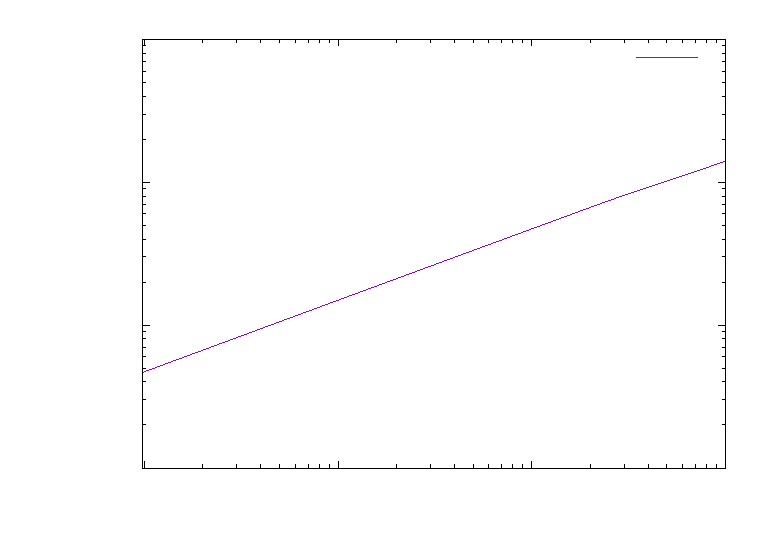
\includegraphics{TransportCvg}}%
    \gplfronttext
  \end{picture}%
\endgroup
}
	\caption{Illustration de l'étude de convergence pour l'équation de transport}
	\label{fig:TransportCvg}
\end{figure}

\noindent Le taux (ou l'ordre) de convergence estimé est donné soit par la pente de la courbe de la figure \ref{fig:TransportCvg}, soit par la formule $$ \text{ordre} \approx \frac{\text{log}\left(\frac{\text{Err}(N)}{\text{Err}(2N) }\right)}{\text{log}(2)}. $$ Un calcul avec $N=5000$ nous donne un ordre de convergence proche de \textbf{0.50}. Ceci indique que le schéma de Godunov converge avec une vitesse de l'ordre de $\sqrt{N}$\footnote{Cet ordre de convergence est indiqué pour les conditions aux limites et initiales imposées par le problème.}.

%-------------------------------------------------------------------------------

\subsection*{Question 5.}
\begin{problem}
	Vérifions numériquement que le schéma devient instable lorsque la condition de CFL n'est pas satisfaite. Traçons un exemple lorsque $c \Delta t / \Delta x > 1$ et proche de $1$.
\end{problem}

\subsection*{Réponse}
Comme précédemment, on prend $L = 2$, $T=0.7$, $c=1$ et $N=1000$. Le coefficient $cfl$ tel que $\Delta t = cfl \times \dfrac{\Delta x}{c}$ est pris égal $1.5, 1.01$ et $0.999$.

\begin{figure}[H]
	\centering
	\begin{subfigure}[b]{0.45\textwidth}
		\centering
		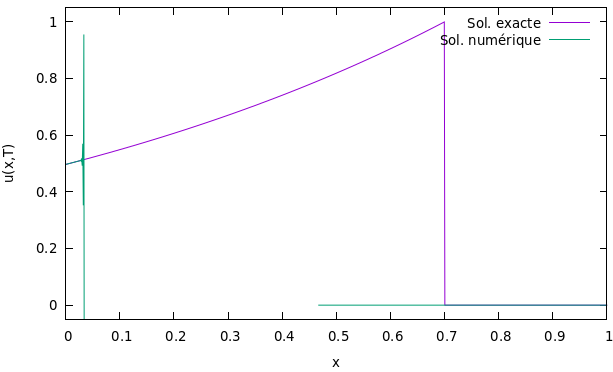
\includegraphics[width=\textwidth]{TransportCFL15.png}
		\caption{$cfl=1.5$}
		\label{fig:TransportCFLa}
\end{subfigure}
	% \hfill
	\begin{subfigure}[b]{0.45\textwidth}
		\centering
		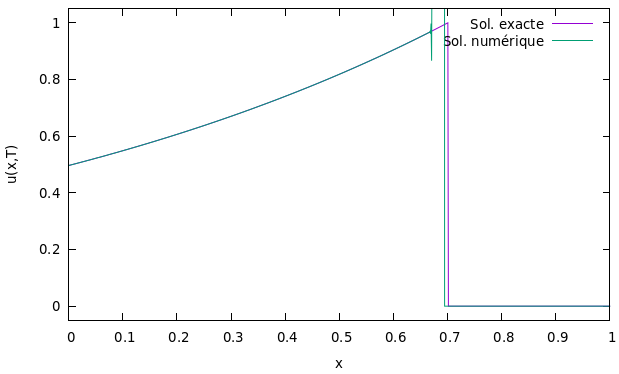
\includegraphics[width=\textwidth]{TransportCFL101.png}
		\caption{$cfl=1.01$}
		\label{fig:TransportCFLb}
	\end{subfigure}
	% \hfill
	\begin{subfigure}[b]{0.45\textwidth}
		\centering
		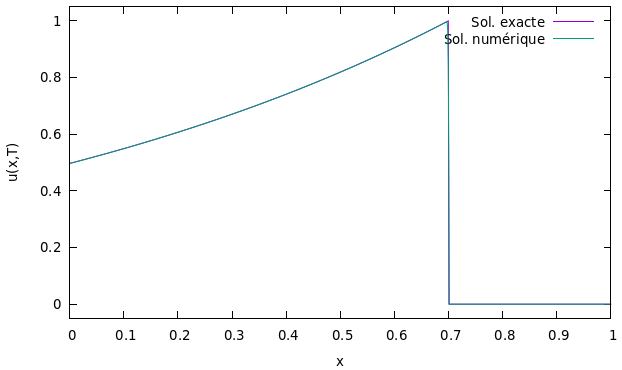
\includegraphics[width=\textwidth]{TransportCFL0999.png}
		\caption{$cfl=0.999$}
		\label{fig:TransportCFLc}
	\end{subfigure}
	% \hfill
	\captionsetup{justification=centering}
	\caption{Vérification numérique de l'instabilité de l'équation de transport}
\end{figure}

\noindent On vérifie ainsi que le schéma est instable lorsque la condition CFL n'est pas satisfaite (figures \ref{fig:TransportCFLa} et \ref{fig:TransportCFLb}). Par contre, lorsque la condition est vérifiée et le coefficient $cfl$ est très proche de $1$, la solution obtenue est considérablement meilleure qu'avec un coefficient $cfl$ plus bas, pour la même taille de maillage ($N = 1000$). On peut observer ceci en comparant les figures \ref{fig:TransportCFLc} (où $cfl=0.999$) et \ref{fig:Transportb} (où $cfl=0.5$).



%----------------------------------------------------------------------------------------
%	ASSIGNMENT CONTENT - SECTION 2
%----------------------------------------------------------------------------------------

\vspace*{2cm}

\section{Résolution numérique de l'équation de Burgers}

\subsection*{Question 1.}
\begin{problem}
	Calculer la solution de Lax du problème suivant.
	\begin{align*}
		% \begin{dcases}
			\partial_t u + \partial_x (u^2/2) &= 0, \qquad x \in ]-1, 2[, \quad t >0 \\
			u(0, t) &= 1 \\
			u(x, 0) &= 
			\begin{dcases}
				1 \hquad & \text{si} \hquad x<0 \\	
				1-x \hquad & \text{si} \hquad 0 \leq x \leq 1 \\	
				0 \hquad & \text{si} \hquad x>1
			\end{dcases}
		% \end{dcases}
	\end{align*}
\end{problem}


\subsection*{Réponse}

Ce problème se réécrit sous la forme $\partial_t u + \partial_x f(u) = 0$, avec $f: u \mapsto \frac{u^2}{2}$.

\noindent Considérons la courbe caractéristique $t \mapsto {x(t) \choose t}$ sur laquelle la solution $u$ est constante i.e. $u(x,t) = u(x(t), t) = \text{Cste}$.

\noindent Ceci donne 
$$
\frac{d}{dt} u(x(t), t) = \left( \frac{\partial u}{\partial t} + x^\prime(t) \frac{\partial u}{\partial x}  \right)(x(t), t) = 0 
$$

\noindent Par comparaison avec l'équation de Burgers qui s'écrit encore sous la forme 
$$ 
\left( \frac{\partial u}{\partial t} + u(x(t),t) \frac{\partial u}{\partial x}  \right)(x(t), t) = 0$$
on déduit que suivant les courbes caractéristiques, on a $x^\prime(t) = u(x(t), t) = \text{Cste}$. On peut donc écrire $$ x^\prime(t) = u(x(0),0) $$ 
% $$= u_0(x(0)) \hquad \text{avec} \hquad u_0: x \in ]-1,2[ \hquad \mapsto \hquad u(x,0)$$.
Distinguons à présent les différents cas possibles d'abscisses à l'origine de la caractéristique:
\begin{itemize}
	\item Si   $ \hquad x(0) < 0, \hquad$ alors
	$$x^\prime(t) = u(x(0),0) = 1 \hquad \Longrightarrow \hquad x(t) = t+x(0) \hquad \Longrightarrow \hquad x(0)=x(t)-t $$
	Il s'en suit que pour $x-t<0$, on a 
	\begin{align*}
		u(x,t) &= u(x(t), t) = \text{Cste} \\
		&= u(x(0),0)  \\
		&=1
	\end{align*}

	\item Si   $\hquad 0 \leq x(0) \leq 1, \hquad$ alors
	$$x^\prime(t) = u(x(0),0) = 1-x(0) \hquad \Longrightarrow \hquad x(t) = (1-x(0))t+x(0) \hquad \Longrightarrow \hquad x(0) = \frac{x(t)-t}{1-t} $$
	Il s'en suit que pour $ 0 \leq \dfrac{x-t}{1-t} \leq 1$, on a 
	\begin{align*}
		u(x,t) &= u(x(t), t)\\
		&= u(x(0),0)  \\
		&=1 - \frac{x-t}{1-t} \\
		&= \frac{1-x}{1-t}
	\end{align*}

	\item Si   $\hquad x(0) > 1, \hquad$ alors
	$$x^\prime(t) = u(x(0),0) = 0 \hquad \Longrightarrow \hquad x(t) = x(0) $$
	Il s'en suit que pour $x>1$, on a 
	\begin{align*}
		u(x,t) &= u(x(t), t)\\
		&= u(x(0),0)  \\
		&=0
	\end{align*}

\end{itemize}

\noindent On obtient donc la solution définie sur $]-1,2[ \times ]0,1[ $ par:
\begin{align*}
	u(x, t) &= 
	\begin{dcases}
		1 \hquad & \text{si} \hquad x<t \\	
		\frac{1-x}{1-t} \hquad & \text{si} \hquad 0 \leq \frac{x-t}{1-t} \leq 1 \\	
		0 \hquad & \text{si} \hquad x>1
	\end{dcases}
\end{align*}

% Vérifions qu'elle verifie le critère de Lax au niveux de ses disconuités apparntes. On pose $f: u \mapsto \frac{u^2}{2}$.
% \begin{itemize}
% 	\item En $x=t$, on a $u_{gauche} =u_L = 1 = \frac{1-t}{1-t} =u_R= u_{droite}$, et la vitesse du choc vaut $\sigma = x^\prime(t) = 1$. On a donc $f^\prime(u_{L}) =u_L= \sigma =u_R = f^\prime(u_{R})$.
% 	\item En $x=1$, on a $u_L = \frac{1-1}{1-t} = 0 = u_R$, et la vitesse du choc vaut $\sigma = x^\prime(t) = 0$. On a donc $f^\prime(u_{L}) =u_L= \sigma =u_R = f^\prime(u_{R})$.
% 	\item En $x=0$, la solution trouvée donne $u(x,t) = u_R = 1 $ (car on suppose $t>0$) correspond bien à la condition de Dirichlet $u(0,t)=1$. 
% \end{itemize}
% On conclut donc que la solution trouvée est continue et vérifie le critère de Lax.

\noindent La fonction trouvée est bien définie et \underline{continue} lorsque $ t<1$. Cependant, lorsque $t \geq 1$, les caractéristiques correspondants aux trois cas se croisent. Notre solution sera alors une solution faible si la pente $\sigma$ de la courbe de discontinuité vérifie la relation de Rankine-Hugoniot (voir \cref{fig:IllusBurg}): 
$$
f(u_L) - f(u_R) = \sigma (u_L - u_R) \Longrightarrow \sigma = \frac{u_L + u_R}{2} = \frac{1 + 0}{2} = \frac{1}{2}
$$
La vitesse de choc $\sigma$ vérifie aussi le critère de Lax car $$f^\prime(u_{L}) = 1 > \sigma = \frac{1}{2} > 0 = f^\prime(u_{R}).$$

\noindent En conclusion, la solution au sens de Lax est donnée par:
\begin{itemize}[label=$\blacksquare$]
	\item Lorsque $t<1$, alors:
	\begin{align*}
		u(x, t) &= 
		\begin{dcases}
			1 \hquad & \text{si} \hquad x<t \\	
			\frac{1-x}{1-t} \hquad & \text{si} \hquad 0 \leq \frac{x-t}{1-t} \leq 1 \\	
			0 \hquad & \text{si} \hquad x>1
		\end{dcases}
	\end{align*}
	\item Lorsque $ t \geq 1 $, alors:
	\begin{align*}
		u(x, t) &= 
		\begin{dcases}
			1 \hquad & \text{si} \hquad x<\frac{1}{2}t \\	
			0 \hquad & \text{si} \hquad x>\frac{1}{2}t
		\end{dcases}
	\end{align*}
\end{itemize}

\begin{figure}[h]
	\centering
	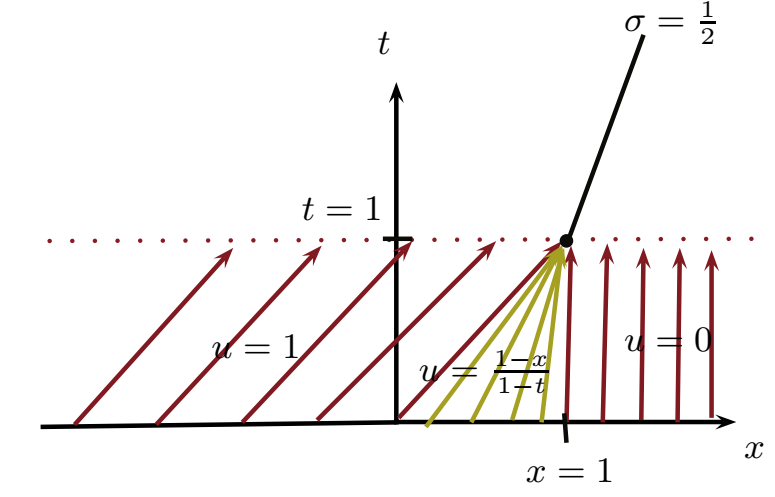
\includegraphics[width=0.5\textwidth]{Burgers1}
	\captionsetup{justification=centering}
	\caption{Illustration de la solution de Lax du problème de Burgers dans l'espace-temps à l'aide des courbes caractéristiques.}
	\label{fig:IllusBurg}
\end{figure}

%-------------------------------------------------------------------------------

\subsection*{Question 2.}
\begin{problem}
	Résoudre le problème de Riemann pour l'équation de Burgers.
	\begin{align}
		\label{Riemann}
		% \begin{dcases}
			\partial_t u + \partial_x (u^2/2) &= 0 \\
			\nonumber u(x, 0) &= 
			\begin{dcases}
				u_L \hquad & \text{si} \hquad x<0 \\	
				u_R \hquad & \text{si} \hquad x>0
			\end{dcases}
		% \end{dcases}
	\end{align}
\end{problem}

\subsection*{Réponse}

Comme précédemment, les courbes  caractéristiques sont les telle que $ x^\prime(t) = u(x(0),0) $. 
On traite tout d'abord les deux cas suivant de façon indépendante:
\begin{itemize}
	\item Si $\hquad x(0) < 0 \hquad$ alors
	$$ x^\prime (t) = u_L \Rightarrow x(t) = u_L t+x(0)$$
	On obtient donc 
	$$ u(x,t) = u_L \hquad \text{pour} \, (x,t) \in D_L, \hquad \text{avec} \, D_L= \left\{ (x,t) \in ]-1,2[ \times \mathbb{R}_+^* \hquad \text{t.q.} \hquad \frac{x}{t} < u_L \right\} $$
	\item Si $\hquad x(0) > 0 \hquad$ alors
	$$ x^\prime (t) = u_R \Rightarrow x(t) = u_R t+x(0)$$
	On obtient donc 
	$$ u(x,t) = u_R \hquad \text{pour} \, (x,t) \in D_R, \hquad \text{avec} \, D_R= \left\{ (x,t) \in ]-1,2[ \times \mathbb{R}_+^* \hquad \text{t.q.} \hquad \frac{x}{t} > u_R \right\} $$
\end{itemize}

Distinguons maintenant deux cas:
\begin{itemize}[label=$\blacksquare$]
	\item Si $u_L > u_R \hquad$ alors les domaines $D_L$ et $D_R$ sont sécants dans l'espace temps; La solution présente donc une discontinuité dont la pente $\sigma$ est donnée par la relation de Rankine-Hugoniot.
	$$
	f(u_L) - f(u_R) = \sigma (u_L - u_R) \Longrightarrow \sigma = \frac{u_L + u_R}{2}
	$$
	On a donc obtenue une solution faible
	$$
	u(x,t) =
	\begin{dcases}
		u_L \hquad & \text{si} \hquad x < \sigma t \\	
		u_R \hquad & \text{si} \hquad x > \sigma t
	\end{dcases}
	$$
	Cette solution vérifie bien le crière de Lax car $f^\prime(u_L) = u_L > \sigma = \frac{u_L + u_R}{2} > u_R = f^\prime(u_R) $.

	%% Une image qui illustre
	\item Si au contraire $u_L < u_R \hquad$, les domaines $D_L$ et $D_R$ sont disjoints dans l'espace temps; la solution faible donnée dans le cas $\hquad u_L > u_R \hquad$ reste applicable, mais ne vérifie plus le critère de Lax.
	
	On construit donc une solution acceptable en exprimant $u$ sur $$D_{milieu} = D_C = \left\{ (x,t) \in ]-1,2[ \times \mathbb{R}_+^* \hquad \text{t.q.} \hquad u_L < \frac{x}{t} < u_R \right\}.$$ On remarque d'entrée que si $u(x,t)$ est solution de l'équation (\ref{Riemann}), alors $u(\lambda x,\lambda  t)$ est aussi solution (pour $\lambda \in \mathbb{R}$). On est donc amené à croire que la solution ne dépend que du rapport $ \xi = x/t$ (i.e $\xi$ est autosimilaire). Posons $u(x,t) = v(\xi)$. On remplace cela dans l'équation (\refeq{Riemann}) pour trouver:
	$$
	\left( \frac{\partial u}{\partial t} + \frac{\partial f(u)}{\partial x}  \right)(x, t) = \left( \frac{\partial v}{\partial t} + \frac{\partial f(v)}{\partial x}  \right)(\xi) = 0 
	$$
	On développe le terme du milieu pour obtenir:
	\begin{align*}
		\left( \frac{\partial v}{\partial t} + \frac{\partial f(v)}{\partial x}  \right)(\xi) &= 	
		\frac{\partial v}{\partial t}(\xi) + f^\prime( v(\xi) ) \frac{\partial v}{\partial x}(\xi) \\
		&=  \frac{\partial v}{\partial \xi}(\xi)\frac{\partial \xi}{\partial t}(t) + v(\xi) \frac{\partial v}{\partial \xi}(\xi) \frac{\partial \xi}{\partial x}(x) \\
		&= \left( -\frac{x}{t^2} + \frac{v(\xi)}{t} \right) v^\prime (\xi)  \\
		&= 0
	\end{align*}
	On remarque que lorsque $v^\prime (\xi) \neq 0$, l'expression de $u$ sur $D_{C}$ peut être obtenue par \footnote{En réalité, $v^\prime(\xi)$ doit être non nul pour avoir des courbes caractéristiques non parallèles et ainsi accomplir la transition de $u_L$ à $u_R$} $$  -\frac{x}{t^2} + \frac{v(\xi)}{t} \Longrightarrow  v(\xi) = u(x,t) = \frac{x}{t} $$

	On est donc amené à considérer la fonction suivante comme candidat pour le problème de Riemann (\ref{Riemann}).
	\begin{align*}
		u(x, t) &= 
		\begin{dcases}
			u_L \hquad & \text{sur} \hquad D_L\\	
			\frac{x}{t} \hquad & \text{sur} \hquad D_C \\	
			u_R \hquad & \text{sur} \hquad D_R
		\end{dcases}
	\end{align*}
	Par construction, $u$ est une solution forte de (\ref{Riemann}) sur $D_L \cup D_C \cup D_R$. En plus, elle est continue au niveau des zones de transition $\frac{x}{t} = u_L$ et $\frac{x}{t} = u_R$. Elle vérifie donc le critère de Lax.
	%% Une image qui illustre
	
\end{itemize}

\noindent En conclusion, la solution du problème de Riemann pour le problème de Burgers est donnée par (voir \cref{fig:IllusRiem}):
\begin{itemize}[label=$\blacksquare$]
	\item Si $ u_L < u_R $, alors la solution est l'onde de choc $$ 	u(x,t) =
	\begin{dcases}
		u_L \hquad & \text{si} \hquad \frac{x}{t} < \frac{u_L + u_R}{2} \\	
		u_R \hquad & \text{si} \hquad \frac{x}{t} \geq \frac{u_L + u_R}{2}
	\end{dcases}$$
	\item Si $ u_L \leq u_R $, alors la solution est l'onde dite de raréfaction $$u(x, t) = 
	\begin{dcases}
		u_L \hquad & \text{si} \hquad \frac{x}{t} < u_L\\	
		u_R \hquad & \text{si} \hquad \frac{x}{t} > u_R \\	
		\frac{x}{t} \hquad & \text{sinon}
	\end{dcases}$$
\end{itemize}

\begin{figure}[h]
	\centering
	\begin{subfigure}[b]{0.4\textwidth}
		\centering
		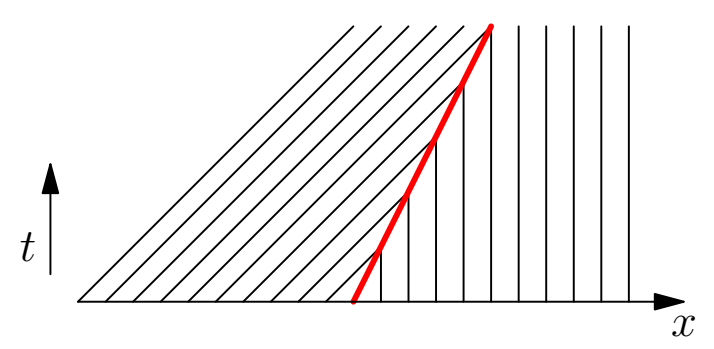
\includegraphics[width=\textwidth]{Riemann1.PNG}
		\caption{$u_L > u_R$}
	\end{subfigure}
	% \hfill
	\begin{subfigure}[b]{0.4\textwidth}
		\centering
		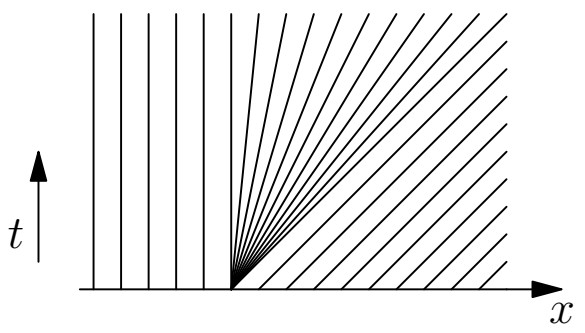
\includegraphics[width=\textwidth]{Riemann2.PNG}
		\caption{$u_L \leq u_R$}
	\end{subfigure}
	% \hfill
	\captionsetup{justification=centering}
	\caption{Illustration de la solution du problème de Riemann à l'aide des courbes caractéristiques}
	\label{fig:IllusRiem}
\end{figure}



\subsection*{Question 3.}
\begin{problem}
	\begin{itemize}
	\item Écrire un programme qui résout le problème (2) par la méthode de Godunov. 
	
	\item Comparer la solution exacte et la solution approchée aux instants $t = 1/2; t = 1; t = 2$ pour diverses finesses de maillage $\Delta x$. 
	
	\item Effectuer une étude de taux de convergence.
	\end{itemize}
\end{problem}

\subsection*{Réponse}

Le code de calcul pour la phase de résolution de l'équation de Burgers par la méthode de Godunov est rigoureusement identique à celui utilisé pour l'équation de transport. Cependant, quelques fonctions doivent êtres adaptées; elles sont toutes données ci-bas.


\begin{lstlisting}[language=C, caption={Flux physique, vitesse maximale, solution du problème de Riemann, et solution exacte pour l'équation de Burgers},breaklines]
void fluxphy(double* w, double* flux) { flux[0] = w[0] * w[0] / 2; }

double lambda_max(double* u) { return fabs(u[0]); }

void riemann(double* a, double* b, double z, double* w) {
	if (a[0] > b[0]) {
		// choc
		double s = (a[0] + b[0]) / 2;
		if (z < s)
			w[0] = a[0];
		else
			w[0] = b[0];
	} else {
		// onde de détente
		if (z < a[0]){
			w[0] = a[0];
		} else if (z > b[0]){
			w[0] = b[0];
		} else
			w[0] = z;
	}
}

void solexacte(double x, double t, double* w) {
	if (x < t){
		w[0] = 1;
	} else if(x > 1) {
		w[0] = 0;
	} else { // if ( 0 <= (x-t)/(1-t) && (x-t)/(1-t) <=1.)
		w[0] = (1-x)/(1-t);
	}
}	
\end{lstlisting}

\noindent Comparons à présent la solution exacte et la solution approchée aux temps indiqués, pour trois finesses de maillages. Les \cref{fig:Burgers1,fig:Burgers2,fig:Burgers3} montrent clairement que les solutions sont meilleures pour des maillages raffinés. Cependant, nous avons vu à la question 1) qu'une solution forte pour ce problème n'existait que pour $t\leq1$. Ceci explique pourquoi le schéma numérique de Godunov ne retrouve pas la solution exacte (faible) que nous avons exprimé à la question précédente; ceci lorsque $t=2$ (\cref{sub@fig:BurgersFaux1,sub@fig:BurgersFaux2,sub@fig:BurgersFaux3}).


\begin{figure}[H]
	\centering
	\begin{subfigure}{0.32\textwidth}
		\centering
		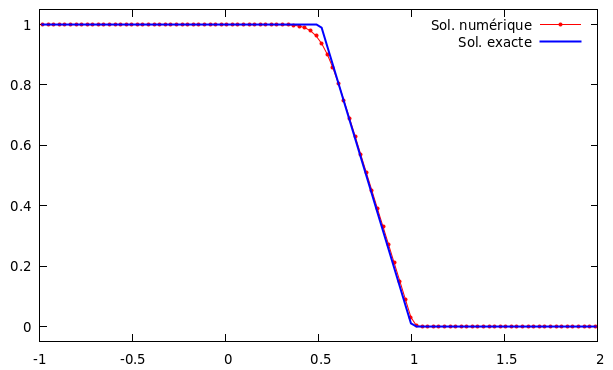
\includegraphics[width=\textwidth]{Burgers2.png}
		\caption{$t=0.5$}
	\end{subfigure}
	\begin{subfigure}{0.32\textwidth}
		\centering
		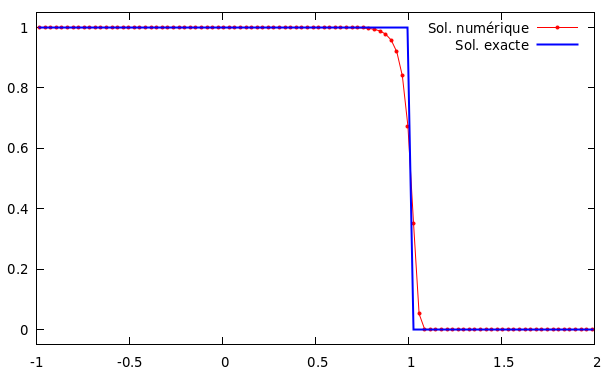
\includegraphics[width=\textwidth]{Burgers3.png}
		\caption{$t=1$}
	\end{subfigure}
	\begin{subfigure}{0.32\textwidth}
		\centering
		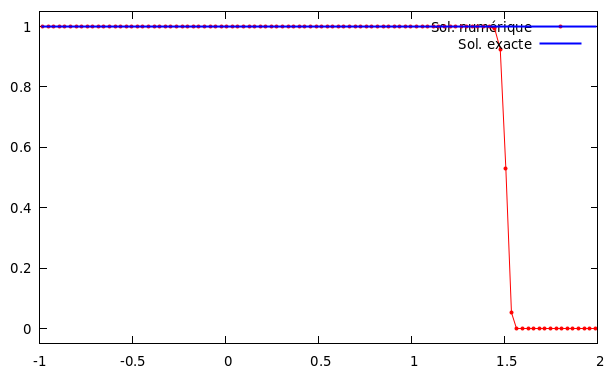
\includegraphics[width=\textwidth]{Burgers4.png}
		\caption{$t=2$}
		\label{fig:BurgersFaux1}
	\end{subfigure}
	\caption{Résolution de l'équation de Burgers par la méthode de Godunov, pour un maillage de taille $N=100$ i.e $\Delta x = 3e-2$.}
	\label{fig:Burgers1}
\end{figure}

\begin{figure}[H]
	\centering
	\begin{subfigure}{0.32\textwidth}
		\centering
		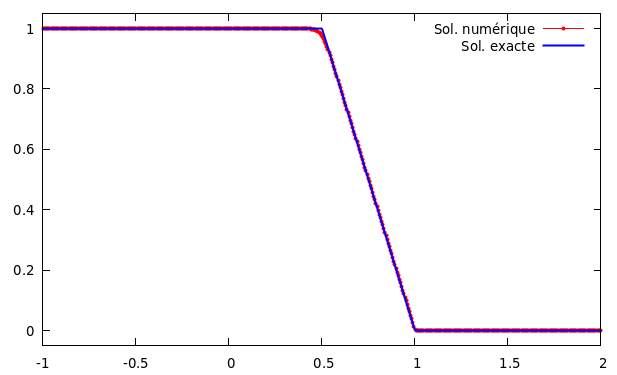
\includegraphics[width=\textwidth]{Burgers5.png}
		\caption{$t=0.5$}
	\end{subfigure}
	\begin{subfigure}{0.32\textwidth}
		\centering
		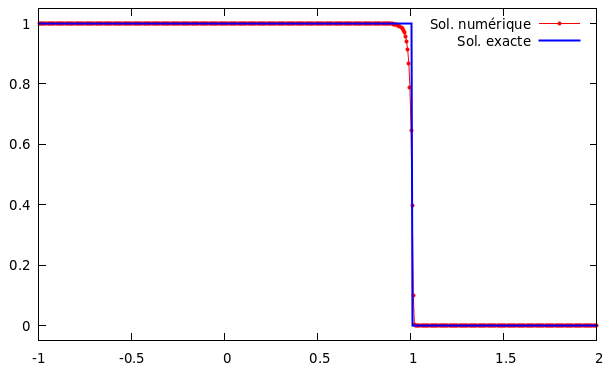
\includegraphics[width=\textwidth]{Burgers6.png}
		\caption{$t=1$}
	\end{subfigure}
	\begin{subfigure}{0.32\textwidth}
		\centering
		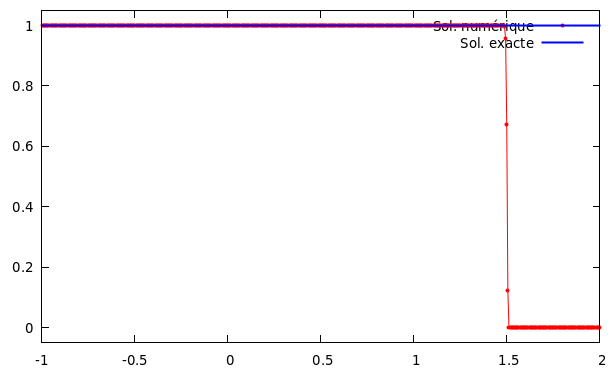
\includegraphics[width=\textwidth]{Burgers7.png}
		\caption{$t=2$}
		\label{fig:BurgersFaux2}
	\end{subfigure}
	\caption{Résolution de l'équation de Burgers par la méthode de Godunov, pour un maillage de taille $N=500$ i.e $\Delta x = 6e-3$.}
	\label{fig:Burgers2}
\end{figure}

\begin{figure}[H]
	\centering
	\begin{subfigure}{0.32\textwidth}
		\centering
		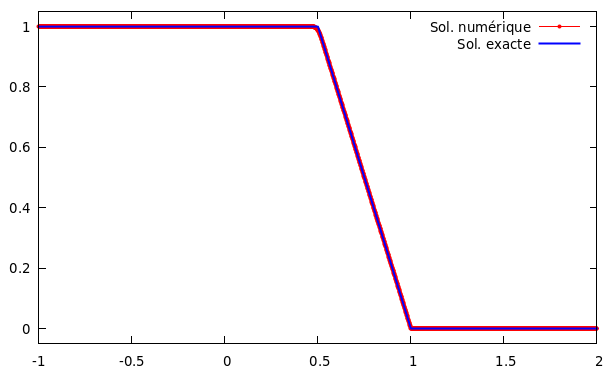
\includegraphics[width=\textwidth]{Burgers8.png}
		\caption{$t=0.5$}
	\end{subfigure}
	\begin{subfigure}{0.32\textwidth}
		\centering
		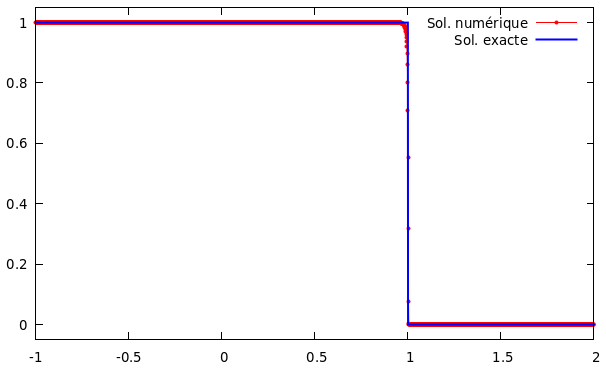
\includegraphics[width=\textwidth]{Burgers9.png}
		\caption{$t=1$}
	\end{subfigure}
	\begin{subfigure}{0.32\textwidth}
		\centering
		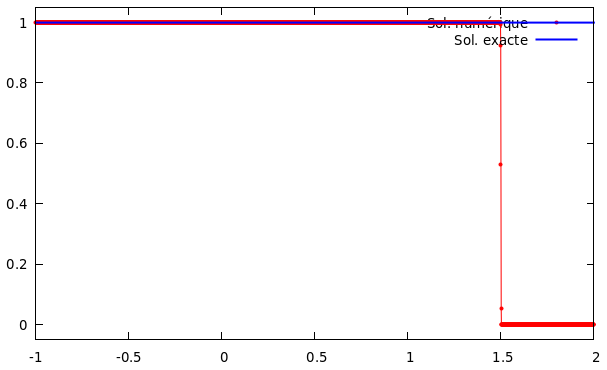
\includegraphics[width=\textwidth]{Burgers10.png}
		\caption{$t=2$}
		\label{fig:BurgersFaux3}
\end{subfigure}
	\caption{Résolution de l'équation de Burgers par la méthode de Godunov, pour un maillage de taille $N=2500$ i.e $\Delta x = 1.2e-3$.}
	\label{fig:Burgers3}
\end{figure}

\noindent Effectuons à présent une étude du taux de convergence, pour les même temps de simulation que précédemment. On obtient la \cref{fig:BurgersConv} qui montre que la meilleure convergence est obtenue pour $t=0.5$, avec un ordre de convergence d'environ $0.99$. Ensuite vient le cas $t=1$, avec un ordre de convergence proche de $0.76$. Enfin, le cas $t=2$ ne saurait converger dû à la non-existence d'une solution forte.

\begin{figure}[H]
	\centering
	\begin{subfigure}{0.32\textwidth}
		\centering
		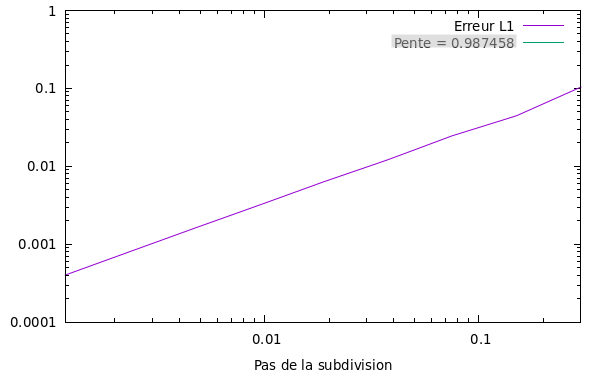
\includegraphics[width=\textwidth]{BurgersConv1.png}
		\caption{$t=0.5$}
	\end{subfigure}
	\begin{subfigure}{0.32\textwidth}
		\centering
		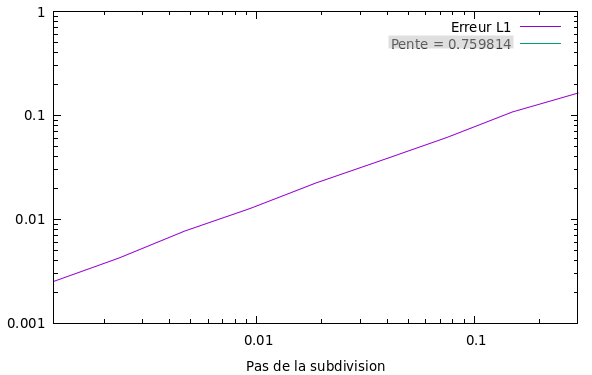
\includegraphics[width=\textwidth]{BurgersConv2.png}
		\caption{$t=1$}
	\end{subfigure}
	\begin{subfigure}{0.32\textwidth}
		\centering
		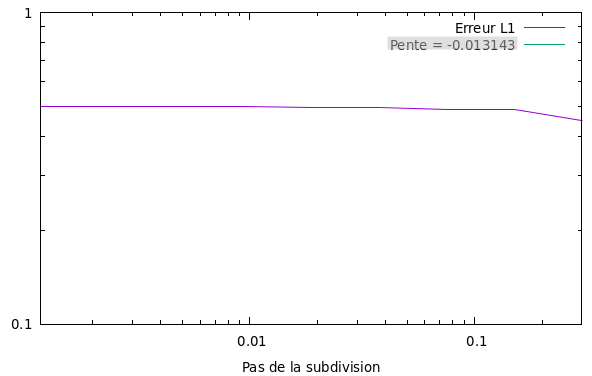
\includegraphics[width=\textwidth]{BurgersConv3.png}
		\caption{$t=2$}
		\label{fig:BurgersFaux4}
\end{subfigure}
	\caption{Étude du taux de convergence pour l'équation de Burgers.}
	\label{fig:BurgersConv}
\end{figure}


\subsection*{Question 4.}
\begin{problem}
	Décrire et programmer la correction MUSCL de van Leer. Vérifier que la précision du schéma est amélioré grâce à une étude de taux de convergence.
\end{problem}

\subsection*{Réponse}


\renewcommand{\sfrac}{\frac}

Rappelons que le schéma de volumes finis en 1D s'écrit pour une maille $i$ à l'itération $n$ comme suit 
\begin{align}
	\label{eq:num1d}
	\frac{w^{n+1}_i - w^n_i}{\Delta t} +  \frac{F^n_{i+\sfrac{1}{2}} - F^n_{i-\sfrac{1}{2}}}{\Delta x} = 0
\end{align}
où les flux numérique aux interfaces sont donnés par 
\begin{align*}
	F^n_{i+\sfrac{1}{2}} = f(w^{n}_{i}, w^{n}_{i+1}) \\
	F^n_{i-\sfrac{1}{2}} = f(w^{n}_{i-1}, w^{n}_{i})
\end{align*}

L'idée de la méthode MUSCL\footnote{L'acronyme MUSCL est mis pour "Monotonic Upstream-centered Scheme for Conservation Laws". Nous décrivons ici la version de cette correction qui prend en compte à la fois les pentes en espace et en temps.} est de remplacer le flux numérique calculé à l'interface $i+\sfrac{1}{2}$ par un flux numérique calculé en des points plus proches de l'interface, et à un pas de temps correspondant. On notera ces points par $w^{n+\sfrac{1}{2}}_{i+\sfrac{1}{2},-}$ et $w^{n+\sfrac{1}{2}}_{i+\sfrac{1}{2},+}$\footnote{Notons qu'un raisonnement similaire est appliqué à l'interface $i-\sfrac{1}{2}$ pour calculer $w^{n+\sfrac{1}{2}}_{i-\sfrac{1}{2},-}$ et $w^{n+\sfrac{1}{2}}_{i-\sfrac{1}{2},+}$.}. On pose alors

\begin{equation}	
	\label{eq:muscl}
	\begin{aligned}
		w^{n+\sfrac{1}{2}}_{i+\sfrac{1}{2},-} &= w^n_i + s^n_i \frac{\Delta x}{2} + r^n_i \frac{\Delta t}{2} \\
		w^{n+\sfrac{1}{2}}_{i+\sfrac{1}{2},+} &= w^n_{i+1} - s^n_{i+1} \frac{\Delta x}{2} + r^n_{i+1} \frac{\Delta t}{2}
	\end{aligned}
\end{equation}

Pour le calcul des pentes en espace $s^n_i$ pour une maille quelconque $i$, on pose:
\begin{align*}
	\alpha = \frac{w^n_{i} - w^n_{i-1}}{\Delta x}, \quad
	\beta = \frac{w^n_{i+1} - w^n_{i}}{\Delta x}, \quad
	\gamma = \frac{w^n_{i+1} - w^n_{i-1}}{2\Delta x}
\end{align*}

et on en déduit
\begin{align*}
	s^n_{i} = \text{minmod}(\alpha, \beta, \gamma)
\end{align*}
où la fonction $\text{minmod}$ est donnée par:
\begin{align*}
	\text{minmod}(\alpha, \beta, \gamma) = 
	\begin{cases}
		\min(\alpha, \beta, \gamma) \qquad &\text{si  } \alpha,\beta,\gamma > 0 \\
		\max(\alpha, \beta, \gamma) \qquad &\text{si  } \alpha,\beta,\gamma < 0 \\
		0 \qquad &\text{sinon  }
	\end{cases}
\end{align*}

Pour le calcul des pentes en temps, on se sert de la loi de conservation décrivant l'équation de Burgers 
$$
\partial_t w + \partial_x f(w) = 0
$$
On prend donc la pente $r^n_i$ telle que 
$$
r^n_i = - f'(w^n_i) s^n_{i} 
$$ 

Les pentes $s^n_{i}$ et $r^n_i$ ayant été calculées, on calcule le flux numérique aux points $w^{n+\sfrac{1}{2}}_{i+\sfrac{1}{2},-}$ et $w^{n+\sfrac{1}{2}}_{i+\sfrac{1}{2},+}$ grâce à l'\cref{eq:muscl}, qu'on applique au schéma numérique. L'\cref{eq:num1d} devient alors
\begin{align}
	\frac{w^{n+1}_i - w^n_i}{\Delta t} +  \frac{F^{n+\sfrac{1}{2}}_{i+\sfrac{1}{2}} - F^{n+\sfrac{1}{2}}_{i-\sfrac{1}{2}}}{\Delta x} = 0
\end{align}

où
\begin{align*}
	F^{n+\sfrac{1}{2}}_{i+\sfrac{1}{2}} = f(w^{n+\sfrac{1}{2}}_{i+\sfrac{1}{2},-}, w^{n+\sfrac{1}{2}}_{i+\sfrac{1}{2},+}) \\
	F^{n+\sfrac{1}{2}}_{i-\sfrac{1}{2}} = f(w^{n+\sfrac{1}{2}}_{i-\sfrac{1}{2},-}, w^{n+\sfrac{1}{2}}_{i-\sfrac{1}{2},+}) 
\end{align*}


En ce qui concerne l'implémentation, le code de calcul précédemment présenté \footnote{La fonction de résolution par la méthode de Godunov simple est la même pour l'équation de transport, et pour l'équation de Burgers.} doit être ajusté. En effet, nous devons rajouter les pentes lors de la résolution du système. On obtient le code de calcul pour la fonction $\verb|godunov_solve|$ ci-bas.

\begin{lstlisting}[language=C, caption={Fonction de résolution du problème de Burger par un schéma de Godunov, auquel on applique la correction MUSCL},breaklines]
void godunov_solve(godunov* gd, double tmax){
	double tnow = 0;
	int m = gd->m;
	while (tnow < tmax) {
		double vmax = 0;
		// calcul de la vitesse max
		for (int i = 0; i < gd->N + 2; i++) {
			double vloc = lambda_max(gd->un + m * i);
			vmax = vmax > vloc ? vmax : vloc;
		}
		// Calcul des pentes pour MUSCL
		double si[gd->N+1], ri[gd->N+1];
		for (int i = 1; i < gd->N + 1; i++) {
			double alpha = (gd->un[i] - gd->un[i-1])/gd->dx;
			double beta = (gd->un[i+1] - gd->un[i])/gd->dx;
			double gamma = (gd->un[i+1] - gd->un[i-1])/(2.0*gd->dx);
			si[i] = minmod(alpha, beta, gamma);
			ri[i] = - gd->un[i] * si[i];
		}
		gd->dt = gd->cfl * gd->dx / vmax;
		for (int i = 1; i < gd->N + 1; i++) {
			double flux[m];
			// Application de MUSCL avec la droite
			double uL[1] = {gd->un[i] + si[i]*gd->dx/2.0 + ri[i]*gd->dt/2.0};
			double uR[1] = {gd->un[i+1] - si[i+1]*gd->dx/2.0 + ri[i+1]*gd->dt/2.0};
			fluxnum(uL, uR, flux);
			for (int iv = 0; iv < m; iv++) {
				gd->unp1[i * m + iv] =
					gd->un[i * m + iv] - gd->dt / gd->dx * flux[iv];
			}
			// Application de MUSCL avec la gauche
			uL[0] = gd->un[i-1] + si[i-1]*gd->dx/2.0 + ri[i-1]*gd->dt/2.0;
			uR[0] = gd->un[i] - si[i]*gd->dx/2.0 + ri[i]*gd->dt/2.0;
			fluxnum(uL, uR, flux);
			for (int iv = 0; iv < m; iv++) {
				gd->unp1[i * m + iv] += gd->dt / gd->dx * flux[iv];
			}
		}
		// mise à jour
		tnow += gd->dt;
		// conditions aux limites
		int i = 0;
		solexacte(gd->xi[i], tnow, gd->unp1 + i * m);
		i = gd->N + 1;
		solexacte(gd->xi[i], tnow, gd->unp1 + i * m);
		// Pour l'iteration suivante
		memcpy(gd->un, gd->unp1, (gd->N + 2) * m * sizeof(double));
	}
	gd->tfin = tnow;
}	
\end{lstlisting}


\noindent Pour tester notre programme, nous reprenons l'étude faite à la question précédente. Les résultats sont présentés aux \cref{fig:Muscl1,fig:Muscl2,fig:Muscl3}. En les comparant aux \cref{fig:Burgers1,fig:Burgers2,fig:Burgers3}, on remarque immédiatement une meilleure approximation numérique, particulièrement perceptible pour un maillage grossier $N=100$.

\begin{figure}[H]
	\centering
	\begin{subfigure}{0.32\textwidth}
		\centering
		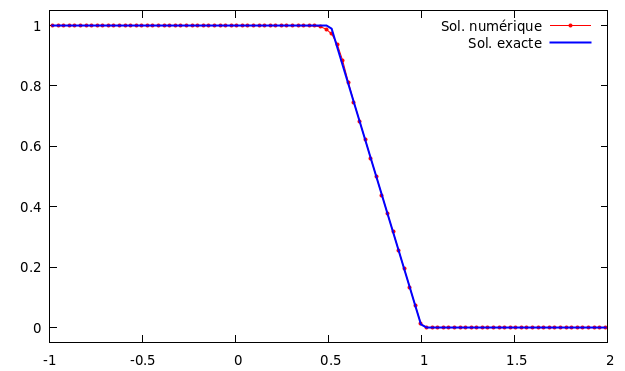
\includegraphics[width=\textwidth]{Muscl2.png}
		\caption{$t=0.5$}
	\end{subfigure}
	\begin{subfigure}{0.32\textwidth}
		\centering
		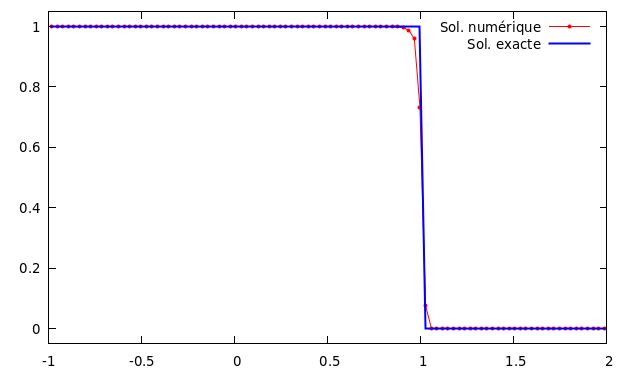
\includegraphics[width=\textwidth]{Muscl3.png}
		\caption{$t=1$}
	\end{subfigure}
	\begin{subfigure}{0.32\textwidth}
		\centering
		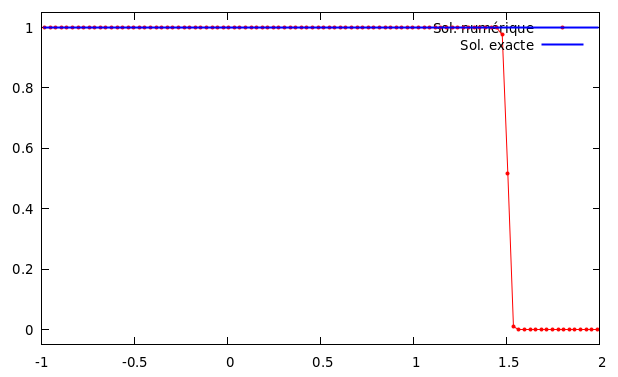
\includegraphics[width=\textwidth]{Muscl4.png}
		\caption{$t=2$}
		\label{fig:MusclFaux1}
	\end{subfigure}
	\caption{Application de la correction de MUSCL au schéma de Godunov, pour un maillage de taille $N=100$ i.e $\Delta x = 3e-2$.}
	\label{fig:Muscl1}
\end{figure}

\begin{figure}[H]
	\centering
	\begin{subfigure}{0.32\textwidth}
		\centering
		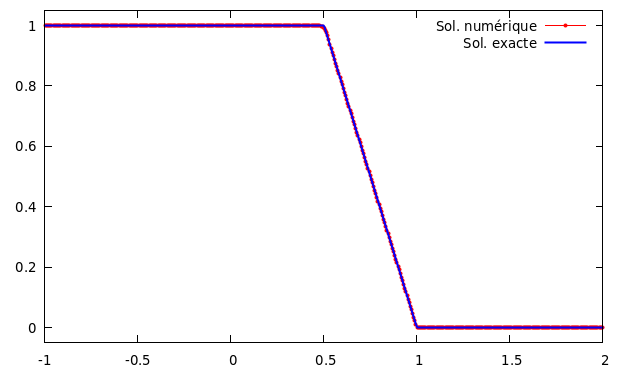
\includegraphics[width=\textwidth]{Muscl5.png}
		\caption{$t=0.5$}
	\end{subfigure}
	\begin{subfigure}{0.32\textwidth}
		\centering
		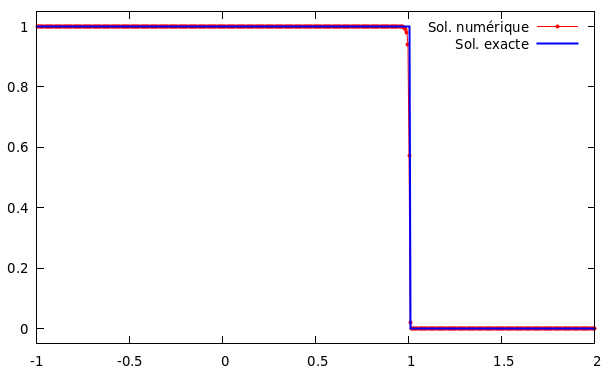
\includegraphics[width=\textwidth]{Muscl6.png}
		\caption{$t=1$}
	\end{subfigure}
	\begin{subfigure}{0.32\textwidth}
		\centering
		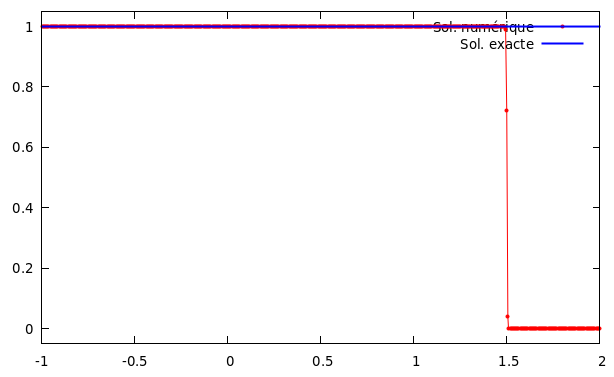
\includegraphics[width=\textwidth]{Muscl7.png}
		\caption{$t=2$}
		\label{fig:MusclFaux2}
	\end{subfigure}
	\caption{Application de la correction de MUSCL au schéma de Godunov, pour un maillage de taille $N=500$ i.e $\Delta x = 6e-3$.}
	\label{fig:Muscl2}
\end{figure}

\begin{figure}[H]
	\centering
	\begin{subfigure}{0.32\textwidth}
		\centering
		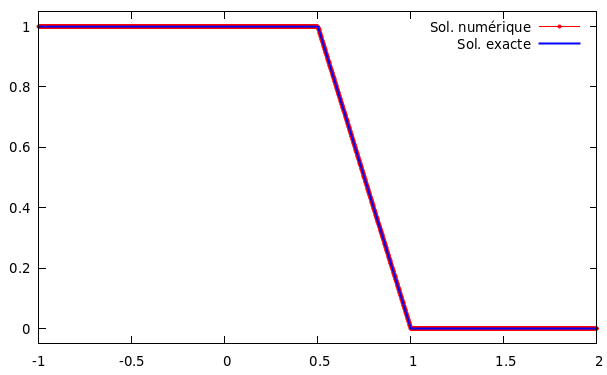
\includegraphics[width=\textwidth]{Muscl8.png}
		\caption{$t=0.5$}
	\end{subfigure}
	\begin{subfigure}{0.32\textwidth}
		\centering
		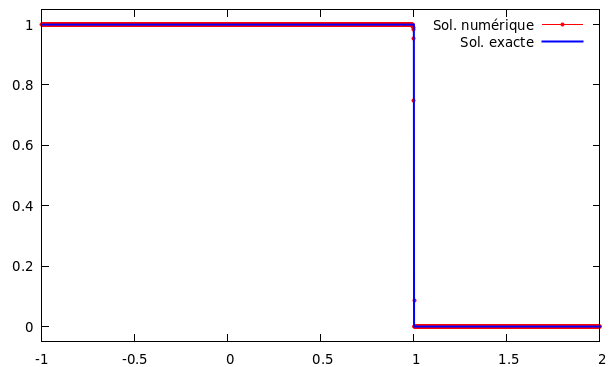
\includegraphics[width=\textwidth]{Muscl9.png}
		\caption{$t=1$}
	\end{subfigure}
	\begin{subfigure}{0.32\textwidth}
		\centering
		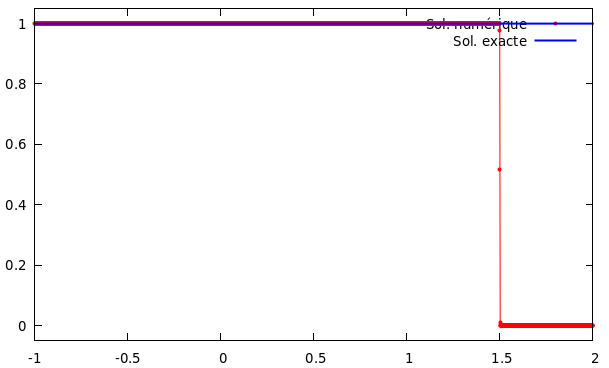
\includegraphics[width=\textwidth]{Muscl10.png}
		\caption{$t=2$}
		\label{fig:MusclFaux3}
\end{subfigure}
	\caption{Application de la correction de MUSCL au schéma de Godunov, pour un maillage de taille $N=2500$ i.e $\Delta x = 1.2e-3$.}
	\label{fig:Muscl3}
\end{figure}


\noindent L'étude du taux de convergence permet de constater la précision supérieure de la correction MUSCL de van Leer. Hormis le cas $t=2$ qui est aberrant, on a, comparé à \cref{fig:BurgersConv}, des meilleures pentes. Ces pentes sont observables sur la figure \cref{fig:MusclConv} et un récapitulatif présenté au \cref{tab:burger}. Il est intéressant de constater qu'en général, le problème de Burgers, bien qu'il soit non-linéaire, converge plus rapidement que le problème de transport (cf. \cref{table:Transport}).

\begin{figure}[H]
	\centering
	\begin{subfigure}{0.32\textwidth}
		\centering
		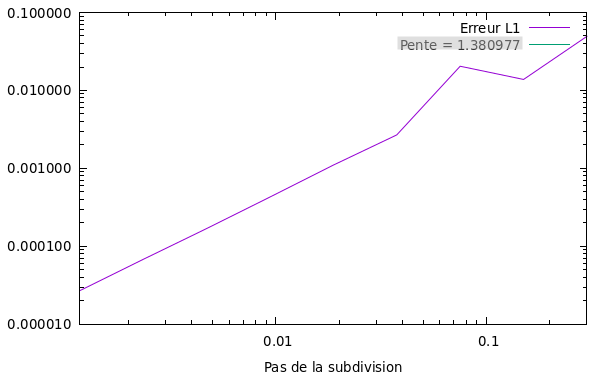
\includegraphics[width=\textwidth]{MusclConv1.png}
		\caption{$t=0.5$}
	\end{subfigure}
	\begin{subfigure}{0.32\textwidth}
		\centering
		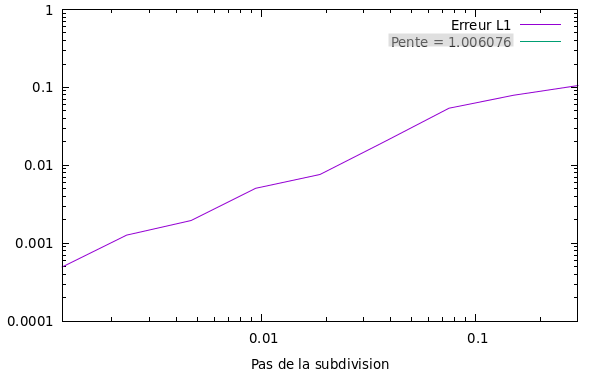
\includegraphics[width=\textwidth]{MusclConv2.png}
		\caption{$t=1$}
	\end{subfigure}
	\begin{subfigure}{0.32\textwidth}
		\centering
		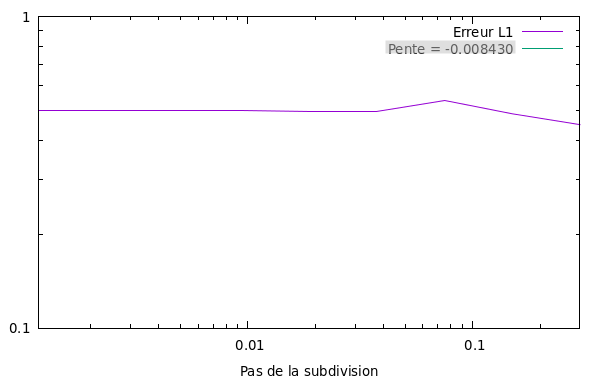
\includegraphics[width=\textwidth]{MusclConv3.png}
		\caption{$t=2$}
		\label{fig:MusclFaux4}
\end{subfigure}
	\caption{Étude du taux de convergence de la méthode de Godunov avec la correction MUSCl.}
	\label{fig:MusclConv}
\end{figure}

\begin{table}[h!]
    \centering
    \begin{tabular}{l c c}
        \toprule
        \tabhead{Temps} & \tabhead{Godunov Simple} & \tabhead{Correction MUSCL} \\
        \midrule
        \tabhead{$t=0.5$} & 0.9875 & 1.3810 \\
        \tabhead{$t=1$} & 0.7598 & 1.0060 \\
        \tabhead{$t=2$} & -0.0131 & -0.0084 \\
        \bottomrule\\
    \end{tabular}
	\caption{Observation de l'amélioration de l'ordre de convergence avec la correction MUSCL. Le cas $t=2$ est aberrant et n'intervient pas dans nos interprétations.}
	\label{tab:burger}
\end{table}



\end{document}
